%%
%% 研究報告用スイッチ
%% [techrep]
%%
%% 欧文表記無しのスイッチ(etitle,jkeyword,eabstract,ekeywordは任意)
%% [noauthor]
%%

%\documentclass[submit,techreq]{ipsj}
\documentclass[submit,techreq,jkeyword,noauthor]{ipsj}

\usepackage[dvipdfmx]{graphicx}
\usepackage{bmpsize}
\usepackage{latexsym}

\def\Underline{\setbox0\hbox\bgroup\let\\\endUnderline}
\def\endUnderline{\vphantom{y}\egroup\smash{\underline{\box0}}\\}
\def\|{\verb|}

\newcommand{\TED}{\textrm{TED}}
\newcommand{\TEDMED}{\textrm{TEDMED}}
\newcommand{\TEDx}{\TED${}^{\textrm{x}}$}
\newcommand{\TEDxTokyo}{\TEDx\textrm{Tokyo}}
\newcommand{\TEDxKyoto}{\TEDx\-\textrm{Kyoto}}
\newcommand{\TEDxSendai}{\TEDx\textrm{Sendai}}
\newcommand{\TEDxParis}{\TEDx\textrm{Paris}}
\newcommand{\TEDxAlcatraz}{\TEDx\textrm{Alcatraz}}
\newcommand{\TEDxReset}{\TEDx\-\textrm{Reset}}

\newcommand{\TEDtitle}{\textbf{TED}}
\newcommand{\TEDxtitle}{\TEDtitle${}^{\textbf{x}}$}
\newcommand{\TEDxKyototitle}{\TEDxtitle\textbf{Kyoto}}

\setcounter{巻数}{0}%vol53=2012
\setcounter{号数}{0}
\setcounter{page}{1}

\begin{document}

\title{アイディアの共有手段としてのエンタテインメント}

%\etitle{How to Prepare Your Paper for IPSJ Journal \\
%(version 2012/10/12)}

\affiliate{OsakaU}{大阪大学\\
Osaka University, Suita, Osaka 565-0871, Japan}

\affiliate{KUFS}{京都外国語大学\\
Kyoto University of Foreign Studies, Kyoto 615-8558, Japan}

\author{金谷 一朗}{Ichiroh Kanaya}{OsakaU}[kanaya@pineapple.cc]
\author{ジェイ クラパーキ}{Jay Klaphake}{KUFS}

\begin{abstract}
建築家リチャード・ソウル・ワーマンは1976年に「情報アーキテクチャ」という言葉を作り,
情報における「アーキテクチャ」の必要性を訴えた.
彼が1984年に設立した非営利のカンファレンス\TED\ (Technology, Entertainment, Design) は
彼の情報アーキテクチャの概念を最もよく表した例である.
\TED カンファレンスは元々学術,エンタテインメント,デザイン分野の研究者がアイディアを共有する場であったが,
現在は分野を絞らず,またそのプレゼンテーションフォーマットを\TEDx として外部にライセンスすることで,
広く社会的影響を与えている.本報告では\TED スタイルと呼ばれるワーマンの設計した情報共有のための
アーキテクチャを一例として,アイディアの共有手段としてのエンタテインメントの可能性を探る.
\end{abstract}

% TEDスタイルを本文に入れる

\begin{jkeyword}
555カンファレンス,\TED カンファレンス,アイディア共有,エンタテインメント,プレゼンテーション形式,
情報アーキテクチャ
\end{jkeyword}

\maketitle

\section{はじめに}

% 問題の定義

情報に構造を与え情報を理解しやすくする研究には長い歴史があり,
それは少なくとも紀元前335年のアリストテレスの叙述にまで遡る.\cite{a}

一方で,その起源もまたアリストテレスに遡ることができるサイエンスとテクノロジーは人類共有の財産であるが,
その知見に構造を与え,情報を共有することは必ずしも簡単ではない.
サイエンス,テクノロジーは数学という高度な抽象度と正確性を持つ道具を駆使するため,
他の学問分野と比較しても一般に「敷居が高い」からである.

学問,とりわけサイエンスやテクノロジーに関する知見の共有は人類の持続的発展のために特に重要であり,
その試みはガリレオ・ガリレイによる著述を皮切りに,
学会や教育機関などによって無数に行われている.\cite{gg}

近年のエデュテイメント (edutainment) や ``Playful Learning'' は特に子供向け教育を念頭に置いた
活動であるが,それらは子供のみならず一般社会人や専門以外の研究者にも十分親しまれている.
これらの試みの第一義は主体的な学習を強くサポートすることであるが,
情報に構造を与え,学習者が未知の情報を想像しやすくするような工夫も試みに含まれる.\cite{nu,mh}
% これらの試みは iTunes U, Khan Academy, MIT Video などのホスティングサービス上で提供されるコースの多数で試みらている.

本報告は,特に近年のサイエンス,テクノロジー分野の知見を一般に共有するための手段を,
その目的において成功しつつある\TED\ (Technology, Entertainment, Design) カンファレンス 
および\TED から派生した\TEDx イベントを内側から俯瞰することで共有を試みるものである.\cite{sugimoto}


% \section{アイディアの共有とエンタテインメント}

% 未来学者トーマス・フレイ (Thomas Frey) は2030年までに現在存在している仕事(職業)の50\%が
% 技術革新によって消えると2012年に講演を行った.\cite{tf}

% 主体的な学習

% この講演と前後して現代を表す標語として「予測困難な時代」という語が使われるようになり,
% 我が国の文部科学省中央教育審議会は2012年に「予測困難な時代において生涯学び続け、
% 主体的に考える力を育成する大学へ」と題する審議まとめを公開した.
% この審議まとめに貫かれているアイディアは,主体的な学習の重要性である.\cite{mext}

% passion based learning


\section{\TEDtitle カンファレンスの取り組み}

建築家リチャード・ソウル・ワーマン (Richard Saul Wurman) は1976年に「情報アーキテクチャ」という
言葉を作り,情報におけるアーキテクチャの必要性を訴えた.\cite{rsw}

ワーマンは後に\TED カンファレンスを設立することで最もよく知られている.
\TED カンファレンスは,元々はテクノロジー,デザインに関する先進的な話題を,
社会的影響力を持つ少人数のグループで共有するためのカンファレンスであったが,
そのカンファレンスのデザインは現在ではアイディアを共有する手段として優れたものと認識されている.\cite{historyofted}

\subsection{カンファレンスのデザイン}

ワーマンは当時非公開であった\TED カンファレンスを1984年に設立するにあたって,
以下のルールを設けた.
\begin{description}
\item[T-1] 1回の講演のトピックはひとつだけに制限される
\item[T-2] ひとりの講演者の持ち時間は最大18分であり,一般にはより短い持ち時間のみが与えられる
\item[T-3] 質疑応答の時間は一部の例外を除いて用意されず,発表後の交流会が質疑応答の時間にあてられる
\item[T-4] 講演者は挨拶,自己紹介を行わず,講演のアウトラインを冒頭に話すことも無い
\item[T-5] スライドやビデオの使用は推奨される
\item[T-6] ポインタは使用されない
\item[T-7] ポディウムは推奨されない
\end{description}
これらのルールがワーマンが講演に与えた情報アーキテクチャである.

ワーマンは過去の著名な講演の殆どが18分以内であることを根拠に(神経科学の知見からではなく)
講演の最大長を決定したと考えられる.\cite{cg}

2001年にワーマンの後を受けた\TED キュレータである
クリス・アンダーソン (Chris Anderson) は以下のように述べ,講演時間の適切さを強調している.\cite{cgweb}
\begin{quote}
It [18 minutes] is long enough to be serious and short enough to hold people's attention.
It turns out that this length also works incredibly well online. It's the length of a 
coffee break. So, you watch a great talk, and forward the link to two or three people. 
It can go viral, very easily. The 18-minute length also works much like the way Twitter 
forces people to be disciplined in what they write. By forcing speakers who are used to 
going on for 45 minutes to bring it down to 18, you get them to really think about what 
they want to say. What is the key point they want to communicate? It has a clarifying 
effect. It brings discipline.
\end{quote}

講演の質疑応答時間を削っているのは,\TED カンファレンスが発表者と聴講者との十分な交流に力を注いでいる
ためである.\TED カンファレンスではおよそ5日間のカンファレンスに対し参加者を1,000人以下に絞っており,
またセッション間の交流時間を毎回1時間以上とることで,発表者,聴講者および聴講者同士の交流時間を十分に
確保するようにしている.

挨拶,自己紹介の排除は,トピックをアイディアに集中させるためであり,
また講演そのものに不必要なコンテクストを残さないための措置である.

ポインタおよびポディウムの非推奨はひとつの理由に基づく.ポディウムの存在は講演者と聴講者の間に文字通り壁を
作るものであり,ワーマンによれば講演においては避けるべきものである.
ポディウムが無い場合,映像を送り出す装置(PC)は手元に無いためポインタはレーザポインタを使って
光学的に重畳することになるが,これは複数スクリーンに対応せず,
また後に述べるビデオアーカイブにもポインタ軌跡を残すことが困難であるため推奨されない.

% 導入,関連研究,原理,実験方法,実験結果,考察,結言と言った理工系論文に見られる章立ては用いられない.
% あえて理工系論文の章立てに当てはめると,\TED で行われる講演は導入部のみである.

\TED カンファレンスは,より広くアイディアを共有するために,次に述べるビデオアーカイブの公開と,
\TEDx と呼ばれるイベント開催ライセンスの発行を行っている.

\subsection{ビデオアーカイブ}

\TED カンファレンスは2006年から「よいアイデアを広めよう (ideas worth spreading)」をスローガンに,
講演のビデオアーカイブをクリエイティブ・コモンズ (CC BY-NC-ND) ライセンス下で無償公開している.
一部の動画は多重ライセンスによる公開を行っている.

\TED ビデオアーカイブは,それが\TED によって制作されたことを示す様々な工夫が盛り込まれている.

講演者は丸い赤絨毯の上に立つ.赤絨毯のサイズは直径2.5[m]から5[m]程度まで毎回異なる.
丸い赤絨毯は視聴者の視覚的な鍵になると同時に,講演者の移動範囲を制限し,
照明およびカメラの照準を決めやすくしている.

ステージには高さが1[m]程度の\TED ロゴが置かれる.
このロゴによって,ビデオアーカイブが確かに\TED によって撮影,編集されたものであることを示すと共に,
類似するカンファレンスとの識別をしやすくしている.

カメラは前方4台,後方1台の合計5台を用いることが多く,前方の1台はクレーン,レールを用いることが多い.
これは一般的な講演の撮影と異なり,小規模な音楽コンサートの撮影に相当する設備である.

また\TED ビデオの特徴として,客席に青い照明をあてることが挙げられる.
講演者の赤絨毯とのカラーのコントラストもあるが,青い照明で客席の照度を上げつつ,
視覚的には暗いという印象を与えるためである.
客席は青照明によって十分な照度が与えられるため,
ビデオアーカイブを見ると聴講者の表情を読み取ることが出来,
聴講者もまたカンファレンスの一部であることが伝わる.

講演者が意図せず18分を超える講演を行った場合でも,ビデオアーカイブは18分に制限される.
これは前節で述べた理由による.

\TED ビデオアーカイブは影響力の強い媒体である.
例えばケン・ロビンソン (Ken Robinson) による講演 ``How schools kill creativity'' は2006年2月に
オンライン公開され,2014年7月までの間に2,700万回以上再生されているほか,
我が国のNHKによるTV放送も行われている.\cite{kr}

% Non commercial

\subsection{\TEDxtitle}

\TEDx とは \TED の「よいアイデアを広めよう (ideas worth spreading)」の精神に基づいて世界各地で
独自に運営されているプログラムである.右肩の「x」は独自に運営されている (independently organized) こと
を示している.

\TED カンファレンスが2009年にパトリック・ニューウェル (Patrick Newel) とトッド・
ポーター (Tod Porter) に independently organized TED event としての\TEDxTokyo ライセンスを
与えたのが\TEDx イベントの始まりである.

\TEDx ライセンス保持者は\TED カンファレンスが提示する\TEDx ライセンス\cite{tedxrules}に
従わねばならない.
\TEDx ライセンスは1年間有効で,授与,更新,譲渡の可否の判断は\TED カンファレンスに委ねられる.
\TEDx イベントは完全に非営利でなければならず,イベント運営者および講演者はボランティアで活動する.
企業ブースの設置など非常に限定的な商利用が\TEDx イベントには認められる.

\TEDx イベントの運営は概ね\TED カンファレンスに準拠したものとなっているが,規模に関する厳しい制約がある.
\TEDx ライセンス保持者が\TED カンファレンスに参加したことが無い場合,
イベント参加者数はボランティア運営者を含めて100名に制限される.

また,原則として講演の 25\% は前述の\TED ビデオアーカイブの上映でなければならい.

\TEDx イベントでの講演は開催後1ヶ月以内にビデオアーカイブを公開することが義務付けられている.
これらのビデオアーカイブは\TED 同様 CC BY-NC-ND ライセンスで公開される.
公開場所は\TED ビデオアーカイブとは異なり YouTube が用いられる.

% Livestream を通したインターネット上の生中継も推奨される.

2013年3月の時点で,平均して1日あたり5件の\TEDx イベントが開催されており,
開催国数は133に達している.\cite{nh,mf}

2014年7月の時点で3万点を超えるビデオアーカイブが公開されている.
\TEDx ビデオアーカイブのうち,優れた講演は\TED キュレータによって選別され \TED ブログに転載される.
特に優れた講演は\TED キュレータによって再編集され\TED ビデオアーカイブとして公開される.\cite{tedxtalksweb}

\begin{figure}[t]
\begin{center}
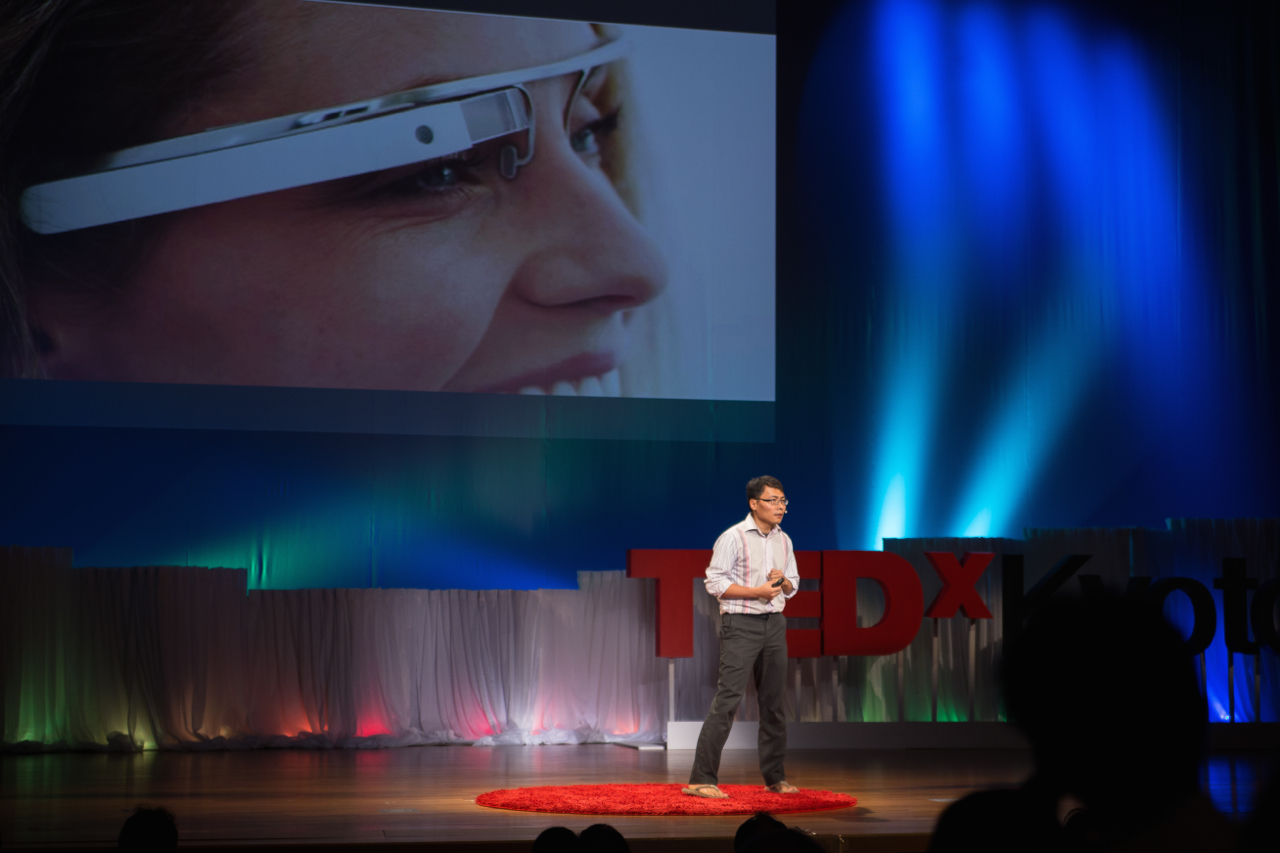
\includegraphics[width=7cm,clip]{tom_chi.png}
\end{center}
\caption{トム・チー (Tom Chi) による Google X の取り組みの紹介\\
(出典: \TEDxKyoto )}
\label{fig:tomchi}
\end{figure}

\subsection{\TEDxKyototitle の取り組み}

\TEDxKyoto はジェイ・クラパーキ (Jay Klaphake) と近藤淳也によって2011年に設立された,京都に拠点を置く\TEDx イベント
運営団体である.\figref{fig:tomchi}に\TEDxKyoto におけるトム・チー (Tom Chi) による講演の様子を示す.

\TEDxKyoto は2012年の最初のイベントから,ワーマンの\TED ルール(T-1からT-7)に加えて,独自のルール\textbf{(T-8)}として,
講演が以下の構造のいずれかに従うようにコーチングを行っている.
\begin{description}
\item[T-8a Chronological] 時系列によって情報を紹介する
\item[T-8b Cause and Effect (Problem and Solution)] まず結果を示し,次に原因を示す(まず問題を示し,次にその解法を示す)
\item[T-8c Contrast and Similarity] 情報Aと情報Bとを比較して,その違いまたは類似性を紹介する
\item[T-8d Classification and Definition] 情報を部分に分割する方法とその結果を紹介する
\end{description}
これらは,英語圏で一般に rhetorical modes と言われるライティングスタイル \cite{cs} のうち,
特に\TEDx 講演に適したものを選択したものである.
サイエンス,テクノロジーに関する発表に関しては T-8b を採用することが多い.

このコーチングを効果的に行うために,\TEDxKyoto は独自の発表規程を設けている.特に重要なものを次に挙げる.
\begin{itemize}
\item 講演者は事前(通常1ヶ月前)に発表用スライド,スクリプトの提出を求められる
\item 専属のコーチが発表内容,発表技術に関するアドバイスを行う
\item スライドは\TEDxKyoto によって再デザインされる
\item 登壇前にリハーサルを行う
\end{itemize}
これらのルールは,主として\TEDxTokyo, \TEDxParis, \TEDxAlcatraz の経験に基づくものである.

セッションは,まず冒頭に強いメッセージ性を持つ講演者を配置し,中間に\TED ビデオアーカイブの上映をはさみ
(これは録画メディアの交換のためにも有用である),最後に情緒的な講演を配置する.
これによって,参加者はセッション中に高いモチベーションを保ち,また一体感を持ったまま交流会の時間を迎える.

講演,セッションに関して,上述のルールを情報アーキテクチャとして組み込むことで,\TEDxKyoto の講演は
品質を保っており,高い評価を得ている.\cite{ml,gr}

2014年6月4日に行われた \TEDxKyoto\ Special Event ``To Boldly Go!'' における
ジョージ・タケイ (George Takei) の講演 ``Power of Pride'' は2014年7月4日に\TED ビデオアーカイブとして
公開され,公開後25日間で約66万回再生されている.\cite{gt}


% \subsection{TEDxライクなイベント}

\section{情報アーキテクチャの必要性}

前節で述べたとおり,情報アーキテクチャを講演に強く埋め込んだ\TED および\TEDxKyoto の
取り組みはアイディア共有の手段として,またエンタテインメントとして高く評価されている.
一方で,意図的に情報アーキテクチャを隠匿したカンファレンスがワーマンによって2012年に提案されている.
このカンファレンスについて次に述べ,改めて情報アーキテクチャの必要性についても述べる.

ワーマンは1998年に医療系に特化した\TED カンファレンスである\TEDMED カンファレンスを設立し,
\TED ルールに縛られないが\TED と趣旨の近いカンファレンスEGを2006年に設立している.
彼は2012年にWWWカンファレンスを主催し,参加者に次のように呼びかけている.\cite{wwwweb}

\begin{quote}
Richard Saul Wurman, creator of the TED (1984-2002), TEDMED (1995-2010) and the eg 
conferences (2006), will celebrate improvised conversation in its most informative manner.

No presentations

No schedule

Simply pairings of amazingly interesting individuals prompted by a question, generating a 
conversation. For 10 minutes to 50 minutes. And so it will go – conversations interlaced 
with threads of improvised music. 
% An astrophysicist and a microbiologist. An actor and a 
% playwright. A jazz musician and a classical one. An energetic exploration of the lost art 
% of conversing.
% 
% Extraordinary individuals,
% minds and musicians in improvised discourse
% 
% A live performance
% 
% A tablet app
% 
% The most innovative moments, the sparks of ideas, and fundamental truths come from 
% conversations between two individuals.
% In the future, the truth will be our most valuable commodity. It is fitting that truth, 
% a commodity that we most value and desire, is amazingly scarce.
% 
% If among all the buttons on your remote control there was one button called truth, 
% wouldn't you push that button?
% 
% WWW is designed to metaphorically provide such a button and create a setting that 
% will allow truth to be revealed.	
$\dots$
\end{quote}

180名が参加したWWWカンファレンスは意図したとおりに機能したが,ワーマンは後にこれが冒険であったことを
% 以下のように
``I was terrified. I wasn't sure it was going to work at all. And then it worked better 
than I thought. So that was a surprise. But it was scary.'' と認めている.\cite{ek}

% \begin{quote}
% I was terrified. I wasn't sure it was going to work at all. And then it worked better 
% than I thought. So that was a surprise. But it was scary.
% \end{quote}

% 555

ワーマンは2014年に555カンファレンスを立ち上げている.
これは世界の5都市で並行して開催される.
各都市では5人の専門家が5週連続して月曜日に講演を行う.
各月曜日の講演に続いて,小規模なミーティングが火曜日に持たれる.
月曜日の講演に関して明確なルールは与えられない.
講演者はワーマンによって予定されているWWW2カンファレンスに参加することになっている.\cite{ek}

WWW/555カンファレンスのような,意図的な情報アーキテクチャの隠匿がアイディア共有の手段として
優れているかどうかは未知であり,またそれが持続可能な取り組みかどうかも本稿執筆時点では未知である.

アイディア共有のための手段としての情報アーキテクチャの組込みは\TED や\TEDxKyoto を通して
高い評価を受けており,またその持続可能性を示しつつある.
WWW/555カンファレンスの取り組みは従来の情報アーキテクチャを排除するものであるが,
情報アーキテクチャそのものを否定するものではない.
これらの知見は,筆者らによる\TEDxKyoto の企画運営の経験に加え,
\TED カンファレンスへの参加や\TEDxTokyo, \TEDxSendai など世界的評価の高いイベントへ
運営者として参加した経験とも合致する.

% 筆者らは\TEDxKyoto の運営を通して,アイディアの共有のためには情報アーキテクチャが有効に機能することを
% 報告する.


\section{おわりに}

本稿では,サイエンス,テクノロジーに関するアイディアの共有という視点から\TED カンファレンスおよび
筆者らが取り組んでいる\TEDxKyoto の事例を紹介した.

\TED および\TEDxKyoto は講演に構造(情報アーキテクチャ)を強く埋め込むことで,
講演にエンタテインメントとしての性質をもたせ,それによってアイディア共有を効果的に行うことを試みている.
\TED はもちろん,\TEDxKyoto の試みも世界的に評価されつつある.

特に筆者らが取り組んでいる\TEDxKyoto での情報アーキテクチャを効果的に共有していくことが,
筆者らの今後の課題である.

\begin{acknowledgment}
本稿執筆にあたり,電子航法研究所の伊藤恵理氏に\TEDxKyoto 講演者の立場から具体的なアドバイスを頂いた.
本稿の内容は\TEDxKyoto メンバである近藤淳也氏,志水良氏,富樫多紀氏,北林功氏,三ツ木隆将氏,川向正明氏,
アンガス・マクレガー氏,長谷川幾与氏,クリスティナ・モアヘッド氏,河原司氏,浅井正嗣氏,
米澤由香里氏,\TEDxKyoto 講演者の河江肖剰氏,\TEDxTokyo メンバである鈴木祐介氏へのインタビューを含む.
% Richard, ...
\end{acknowledgment}

\begin{thebibliography}{10}
\bibitem{a} アリストテレース: 詩学; 岩波書店, 1997.
\bibitem{gg} ガリレオ・ガリレイ: 天文対話; 岩波書店, 1959.
\bibitem{nu} 上田信行, 中原淳: プレイフル・ラーニング; 三省堂, 2012.
\bibitem{mh} Melinda Wenner: \textsl{The Serious Need for Play;} Scientific American, Issue of March 2009, 2009.
\bibitem{sugimoto} Sugimoto CR, Thelwall M, Larivière V, Tsou A, Mongeon P, Macaluso B.: \textsl{Scientists popularizing science: characteristics and impact of TED talk presenters;} PLoS One; 8(4), PMID: 23638069, 2013. 
\bibitem{rsw} Richard Saul Wurman: \textsl{Information Architects;} Graphis Inc., 1997.
\bibitem{historyofted} TED: \textsl{History of TED (online);} \urle{http://bit.ly/history-of-ted} (2014-07-21).
% \bibitem{nn} Nicholas Negroponte: \textsl{Being Digital;} Vintage, 1995.
% Garr
\bibitem{cg} Camine Gallo: \textsl{Talk like TED: The 9 Public-Speaking Secrets of the World's Top Minds;} St. Martin's Press, 2014.
\bibitem{cgweb} Camine Gallo: \textsl{The Science Behind TED's 18-Minute Rule (online);} \urle{http://bit.ly/science-behind-18-minute-rule} (2014-07-21).
\bibitem{kr} Ken Robinson: \textsl{How schools kill creativity;} \urle{http://on.ted.com/e0Kis} (2014-07-21).
\bibitem{tedxrules} TED: \textsl{TEDx rules (online);} \urle{http://bit.ly/tedx-rules} (2014-07-21).
\bibitem{nh} Nathan Heller: \textsl{Listen and Learn;} The New Yorker, 9 July 2012.
\bibitem{mf} Mark Fidelman: \textsl{Here's Why TED and TEDx are So Incredibly Appealing;} Forbes, 19 June 2012.
\bibitem{tedxtalksweb} TED: \textsl{TEDx talks  (online);} \urle{http://tedxtalks.ted.com} (2014-07-21).
\bibitem{cs} Carlota S. Smith: \textsl{Modes of Discourse: The Local Structure of Texts;} Cambridge University Press, 2003.
\bibitem{ml} Michael Lambe: \textsl{To Boldly Go – TEDxKyoto x George Takei \& Patrick Linehan (online);} Deep Kyoto, 4 June 2014, \urle{http://www.deepkyoto.com/?p=10238} (2014-07-21).
\bibitem{gr} Garr Reynolds: \textsl{Presentation Zen Design;} Amazon Digital Service, 2013.
\bibitem{gt} George Takei: \textsl{Why I love a country that once betrayed me (online);} \urle{http://on.ted.com/g0MFO} (2014-07-21).
\bibitem{wwwweb} Richard Saul Wurman: \textsl{WWW conference (online);} \urle{http://bit.ly/www-conference} (2014-07-21).
\bibitem{ek} Emi Kolawole: \textsl{555 Conference: TED creator Richard Saul Wurman discusses his latest gathering (online);} The Washington Post, 30 July 2013, \urle{http://wapo.st/1645gEj} (2014-07-21).
% \bibitem{hs} Hadas Shema: \textsl{The Impact of TED Talks (online);} Scientific American Blogs, ...
\end{thebibliography}


%% 以下は無視されます

\begin{biography}
\profile{m}{情報 太郎}{1970年生.1992年情報処理大学理学部情報科学科卒.
1994年同大大学院修士課程了.同年情報処理学会入社.オンライン出版の研究
に従事.電子情報通信学会,IEEE,ACM 各会員}
%
\profile{n}{処理 花子}{1960年生.1982年情報処理大学理学部情報科学科卒.
1984年同大大学院修士課程了.1987年同博士課程了.理学博士.1987年情報処
理大学助手.1992年架空大学助教授.1997年同大教授.オンライン出版の研究
に従事.2010年情報処理記念賞受賞.電子情報通信学会,IEEE,IEEE-CS,ACM
各会員}
%
\profile{s}{学会 次郎}{1950年生.1974年架空大学大学院修士課程了.
1987年同博士課程了.工学博士.1977年架空大学助手.1992年情報処理大学助
教授.1987年同大教授.2000年から情報処理学会顧問.オンライン出版の研究
に従事.2010年情報処理記念賞受賞.情報処理学会理事.電子情報通信学会,
IEEE,IEEE-CS,ACM 各会員}
%
\end{biography}



\end{document}
